
%% bare_adv.tex
%% V1.4
%% 2012/12/27
%% by Michael Shell
%% See: 
%% http://www.michaelshell.org/
%% for current contact information.
%%
%% This is a skeleton file demonstrating the advanced use of IEEEtran.cls
%% (requires IEEEtran.cls version 1.8 or later) with an IEEE Computer
%% Society journal paper.
%%
%% Support sites:
%% http://www.michaelshell.org/tex/ieeetran/
%% http://www.ctan.org/tex-archive/macros/latex/contrib/IEEEtran/
%% and
%% http://www.ieee.org/

%%***********************************************
\documentclass[12pt,journal,compsoc]{IEEEtran}



\newcommand\MYhyperrefoptions{bookmarks=true,bookmarksnumbered=true,
pdfpagemode={UseOutlines},plainpages=false,pdfpagelabels=true,
colorlinks=true,linkcolor={black},citecolor={black},urlcolor={black},
pdftitle={Bare Demo of IEEEtran.cls for Computer Society Journals},%<!CHANGE!
pdfsubject={Typesetting},%<!CHANGE!
pdfauthor={Michael D. Shell},%<!CHANGE!
pdfkeywords={Computer Society, IEEEtran, journal, LaTeX, paper,
             template}}%<^!CHANGE!

\hyphenation{op-tical net-works semi-conduc-tor}
\usepackage{graphicx}
\graphicspath{ {./images/} }
\usepackage[justification=centering]{caption}
\usepackage{subfig}
\usepackage{mathrsfs}
\usepackage{mathtools}
\DeclarePairedDelimiter\ceil{\lceil}{\rceil}
\DeclarePairedDelimiter\floor{\lfloor}{\rfloor}
\begin{document}

\title{CNN for Single Image Super-Resolution\\ and HEVC Sub-pixel Interpolation}


\author{Yixu Chen,~\IEEEmembership{Electric \& Computer Engineerings} 
% <-this % stops a space
\IEEEcompsocitemizethanks{\IEEEcompsocthanksitem
E-mail: cyx709671676@gmail.com}% <-this % stops a space
\IEEEcompsocitemizethanks{\IEEEcompsocthanksitem
UIN: 627008228}
\thanks{}}


\IEEEtitleabstractindextext{
\begin{abstract}
In HEVC video coding standard, the intre-prediction between picture need sub-pixel level accuracy for motion estimation. HEVC current using 1/4 precision for luminance and 1/8 precision for chrominance. In this work we compare a few convolutional neural networks methods for single image super-resolution and the HEVC's 7 and 8 taps filter for sub-pixel interpolation.

The CNN used for SISR includes Super-Resolution Convolutional Neural Network (SRCNN) and the Efficient Sub-Pixel Convolutional Neural Network (ESPCN). As we will see in the result, the better interpolation we can do, the more compression ratio we can get.
\end{abstract}

\begin{IEEEkeywords}
Single Image Super-Resolution, HEVC, Sub-pixel Interpolation, ESPCN, SRCNN, motion estimation.
\end{IEEEkeywords}}


% make the title area
\maketitle



\IEEEdisplaynontitleabstractindextext

\IEEEpeerreviewmaketitle

\section{Introduction}
\subsection{Image super-resolution}
In computer vision, the super resolution(SR) is a techniques used for recovering high resolution (HR) image from low resolution (LR) image. This problem is highly ill-posed since the detail in LR image is completely lost and there are no single ground truth for the HR images recovered from it. 

It is an inverse problem in mathematics.

\begin{equation} 
\label{eqn_example} 
F(I_h) = I_l
\end{equation}
$F$ is the continuous mapping from the high rank matrix $I_h$ to the low rank matrix $I_l$ . $I_h$ and $I_l$ are the image representation matrices.

Constructing $I_h$ from $I_l$ is to compute the inverse $F^{-1}$. This is an underdetermined inverse problem of which the solution is not unique.

\subsection{Sup-pixel Interpolation}
The interpolation methods we usually used for image upscaling are nearest neighbor, bilinear and bicubic interpolation which are naive super-resolution methods. 

In HEVC, the motion compensation(MC) is used for inter-picture predictive coding. Finding a best motion vector(MV) for a predictive unit in the current frame based on several reference frames and then code the residual can significantly reduce the bitrate.

The location of the reference block is indicated by the MV. In other words, the content inside the current block is assumed to have a translation relationship between the current picture and the reference picture. However, the translation may not be aligned with the pixels, thus simply moving the reference block in integer pixel length is not enough. Therefore, sub-pixel MC is put forward to generate the pixel in the fractional level to serve for prediction. Fig. \ref{fig_1} is an illustration of sub-pixel MC.

\begin{figure}[!t] 
\centering
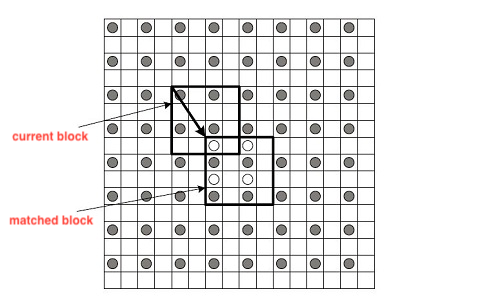
\includegraphics[width=2.5in]{1_ME.png}
\caption{Sub-pixel Motion Compensation}
\label{fig_1}
\end{figure}


Nowadays HEVC using separable 8-tap DCT interpolation filter(DCTIF) for half-sample positions luma interpolation and 7-tap filter for the quarter-sample positions. In contrast to H.264/AVC which adopts a 6-tap finite impulse response filter for half-pixel interpolation and additionally adopts simple linear interpolation for quarter-pixel interpolation.

 Although in HEVC we are using 7 or 8 pixels near the predicted one to do the interpolation. It is still very limited compared to the reception field of neural network method, for example, SRCNN uses 169 pixels in a three layer structure to predicted one pixel.

Due to the non-stationary properties of natural videos, fixed interpolation filters may not work well enough for different videos. In this work we try to implement two different neural network to do super-resolution instead of interpolation.

\section{SRCNN}
\subsection{Networks structure}
Super-Resolution Convolutional Neural Network (SRCNN)\cite{DBLP:journals/corr/DongLHT15} was put forward as the first work of using convolutional neural network to do image super-resolution. It have achieved great result but not fast enough for video. 

In this network, the original low resolution(LR) images are upsampled to the desired size using traditional bicubic interpolation method. And then go through 3 layers of CNN to refine the high frequency detail. It is fully feed-forward convolutional neural network that learns an end-to-end mapping between low and high-resolution images, with little pre-processing or post-processing beyond the optimization.

To map a low resolution image $Y$ to its hight resolution counterpart $X$, first, we upscale $Y$ using bicubic interpolation to the same size as $X$. Then, for each  overlapping patches from it, we extract a set of feature map. Next, a nonlinear mapping is performed to convert low resolution patches from Y into high resolution patches. Finally, these high resolution patches are aggregated into a high resolution image $X'$. We expect $X'$ to be as close as possible to $X$, based on which we can define the loss function for the training process.

\begin{enumerate}
  \item Patch extraction and representation: The first layer of the CNN has $n_1$ filters with kernel size $c \times f_1 \times f_1$ where $c$ is the number of channels and $f_1$ is the spatial size of the kernel. This layer extracts an $n_1$ dimensional feature for each patch. 
  \begin{equation}
  	F_1(Y) = max(0,W_1*Y+B_1)	
  \end{equation}
  $W_1$ and $B_1$ are the filters and biases and $*$ denotes the convolution operation. ReLU is used as the activation function.
  \item Nonlinear mapping: The second layer has $n_2$ filters with size $n_1 \times f_2 \times f_2$ . This layer map each of the $n_1$ dimensional feature to an $n_2$ dimensional one. Conceptually, each of the $n_2$ dimensional feature is a representation of a high-resolution patch.
  \begin{equation}
  	F_2(Y) = max(0,W_2*F_1(Y)+B_2)	
  \end{equation} 
  
  \item Reconstruction: The last convolutional layer produces the final high-resolution image with kernel size $n_2 \times f_3 \times f_3$
  \begin{equation}
  	F(Y) = W_3*F_2(Y)+B_3
  \end{equation}
  \end{enumerate}



\begin{figure*}[!t] 
\normalsize
\centering
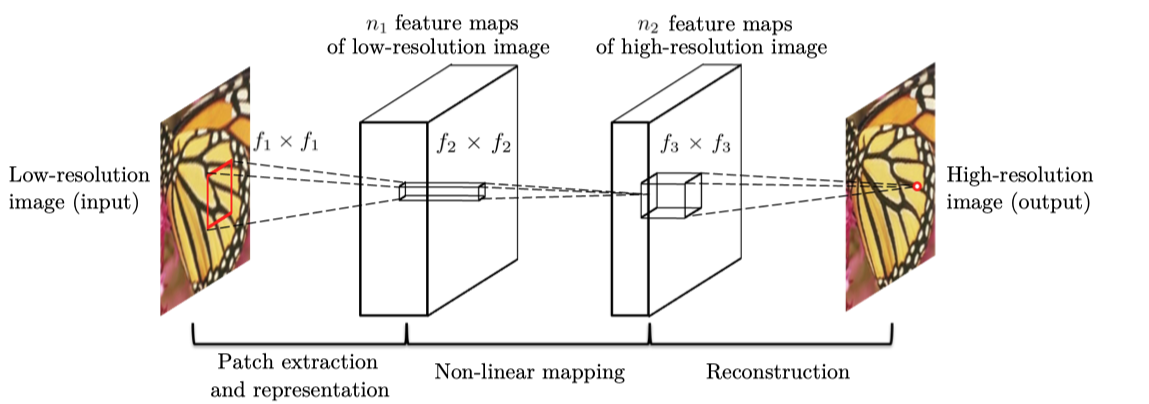
\includegraphics[width=7in]{2_SRCNN.png}
\vspace*{4pt} 
\caption{Sub-pixel Motion Compensation}
\label{fig_2}
\end{figure*}


Fig. \ref{fig_2} is an illustration of SRCNN network structure.

\subsection{Training}

\subsubsection{Data}
We use the benchmark dataset in \cite{DBLP:journals/corr/DongLHT15}. It includes a small training set of 91 images which can be decomposed into many sub-image pairs. 
\begin{enumerate}
  \item Convert the original image from RGB to YCbCr and only use the Y channel.
  \item Then we downsample the HR image to LR image using bicubic method to the scale of $n$.
  \item Crop the LR images into LR sub-images of size $f_{sub} \times f_{sub} \times c$ with the $stride_{lr}$.
  \item Crop the HR images into HR sub-images of size $nf_{sub} \times nf_{sub} \times c$ with the $stride_{hr} = n \times stride_{lr}$
\end{enumerate}
As depicted in the \cite{DBLP:journals/corr/DongLHT15}, The performance of using Y channel is even better than using YCbCr 3 channels as the training may falls into a bad local minimum, due to the inherently different characteristics of the Y and Cb, Cr channels. Here, we use only Y channel.

We tried scale of 3 and 4. For the scale $n = 3$ with the $stride_{lr} = 5$, $stride_{hr} = 15$, $f_{sub} = 11$ we have $19382$ sub-images.
For $n = 4$ with the $stride_{lr} = 5$, $stride_{hr} = 20$,  $f_{sub} = 11$ we have $10087$ sub-images. 
Combine them into sub-image pairs and used as input and ground truth.

\subsubsection{Parameters}
For the SRCNN 9-1-5 network parameters is shown in the Table \ref{table_1}. Here, we use padding to make the network have same size of output. Since we only use Y channel $c = 1$.

For the SRCNN 9-5-5 network, just let $f_2 = 5$, we tried both setting.

\begin{table*}[]
\normalsize
%\renewcommand{\arraystretch}{1.3} 
\caption{SRCNN 9-1-5 network} 
\label{table_1} 
\centering
\begin{tabular}{|l|l|l|l|l|}
\hline
              & filter size   & parameters      & output size & \# of parameters 	\\ \hline
image patches &               & $f_{sub}=11$    & $11*11*1$   & $0$  	\\
    \hline
bicubic upscale &               &    & $33*33*1$   & $0$  	\\ \hline
1st layer     & $9*9*1$       & $f_1=9, n_1=64$ & $33*33*64$  & $5248$ 	\\ \hline
2nd layer     & $1*1*64$      & $f_2=1, n_2=32$ & $33*33*32$  & $2080$ 	\\ \hline
3rd layer     & $5*5*32$      & $f_3=5,n_3=1$   & $33*33*1$   & $801$  	\\ \hline
\end{tabular}
\vspace*{4pt}
\end{table*}


\section{ESPCN}
For ESPCN\cite{DBLP:journals/corr/ShiCHTABRW16}, the upsampling process is realized by deconvolution instead of bicubic interpolation. The network structure is illustrated in Fig. \ref{fig_espcn}.
To avoid upscaling LR image before feeding it into the network. ESPCN first apply a 3 layers convolutional neural network directly to the LR image, and then apply a sub-pixel convolution layer that upscales the LR feature maps to produce the HR image. The calculation is significantly reduced as the feature calculation is done in LR space with less pixels to calculate.

The sub-pixel convolution layer 

ESPCN use periodic shuffling $\mathcal{PS}$ operator in the last layer. Before the last layer, we get $Cr^2$ features and then $\mathcal{PS}$ rearranges a $H\times W \times r^2 C$ tensor to a $Hr \times Wr \times C$ tensor:

\begin{equation} 
\mathcal{PS}(T)_{x,y,c} = T_{\floor*{x/r},\floor*{y/r},Cr \cdot mod(x,r)+C \cdot mod(y,r) + c}
\end{equation}
The parameters of ESPCN is listed in the Table \ref{table_2}.

\begin{table*}[]
\normalsize
\renewcommand{\arraystretch}{1.3} 
\caption{ESPCN network} 
\label{table_2} 
\centering
\begin{tabular}{|l|l|l|l|l|}
\hline
              & filter size   & parameters      & output size & \# of parameters 	\\ \hline
image patches &               & $f_{sub}=11$    & $11*11*1$   & $0$  	\\ \hline
1st layer     & $5*5*1$       & $f_1=5, n_1=64$ & $11*11*64$  & $1664$ 	\\ \hline
2nd layer     & $3*3*64$      & $f_2=3, n_2=32$ & $11*11*32$  & $18464$ 	\\ \hline
3rd layer     & $3*3*32$      & $f_3=3, n_3=9$  & $11*11*9$   & $2601$  	\\ \hline
sub-pixel convolution     &       &   & $33*33*1$   & $0$  	\\ 
	\hline
\end{tabular}
\vspace*{4pt}
\end{table*}

\begin{figure*}[!t]
\normalsize
\centering
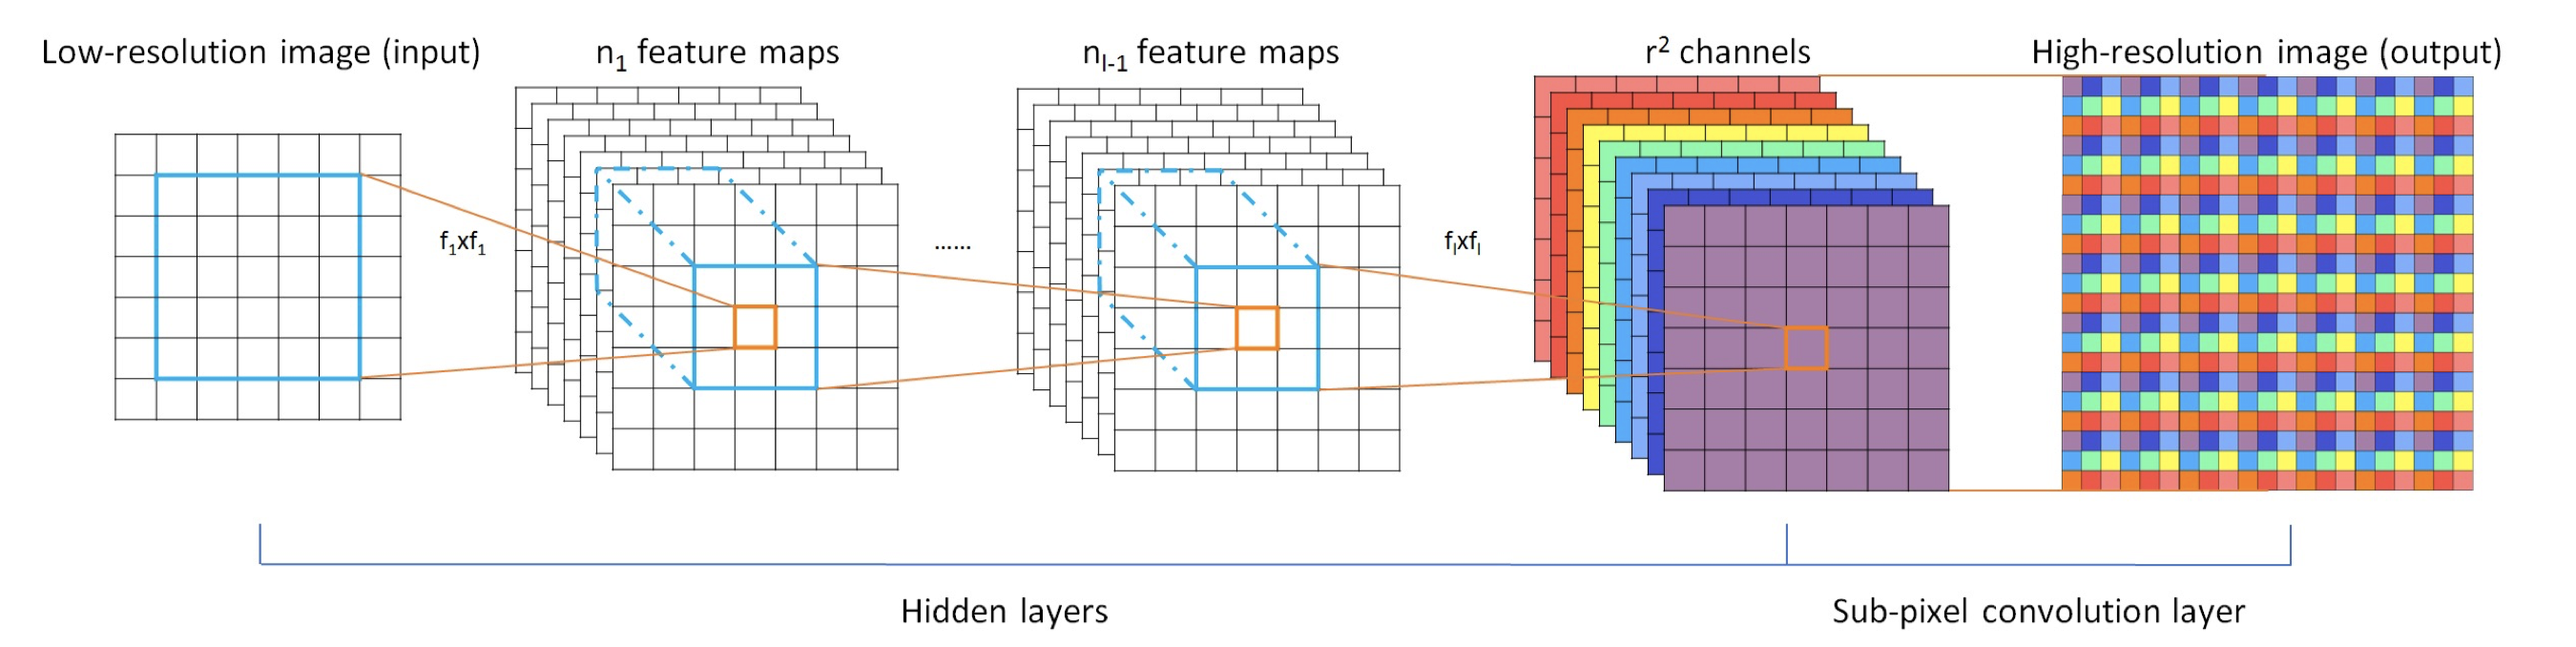
\includegraphics[width=7in]{3_espcn.png}
\vspace*{4pt} 
\caption{ESPCN network structure}
\label{fig_espcn}
\end{figure*}


\section{HEVC sub-pixel interpolation}
The fractional sample interpolation for luma samples in HEVC uses separable application of an eight-tap filter for the half-sample positions and a seven-tap filter for the quartersample positions.

In Fig \ref{hevc}, the positions labeled with upper-case letters, $A_{i,j}$, represent the available luma samples at integer sample locations, whereas the other positions labeled with lower-case letters represent samples at noninteger sample locations, which need to be generated by interpolation.
For detailed implementation, see \cite{6316136} and my code.
\begin{figure}[!t]
\centering
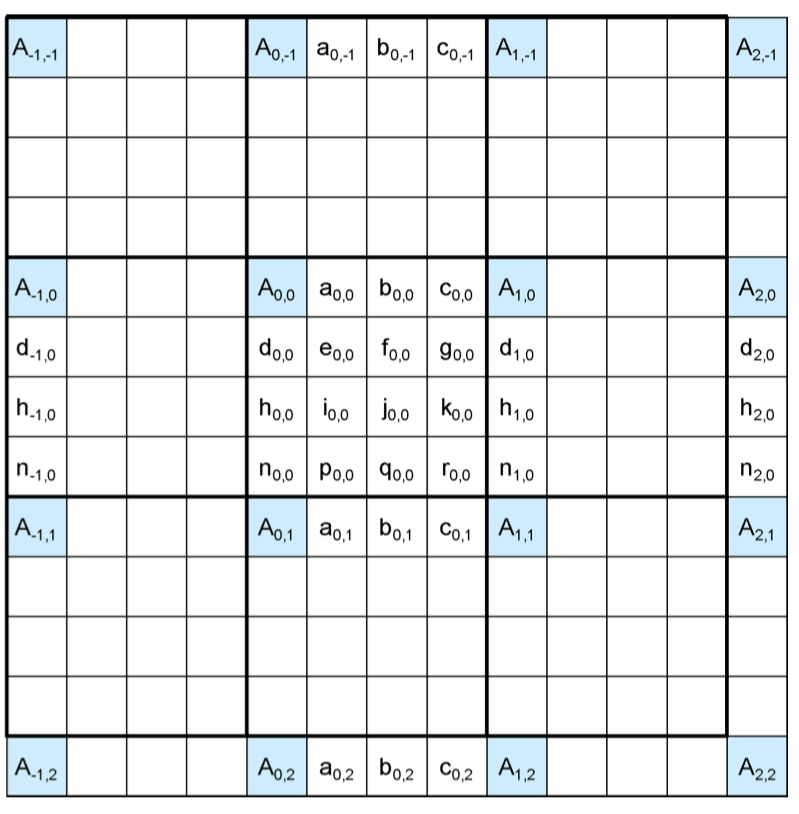
\includegraphics[width=3in]{hevc.png}
\vspace*{4pt} 
\caption{HEVC sub-pixel interpolation}
\label{hevc}
\end{figure}


\section{Result}
\subsection{Training}
We use Mean Squared Error as the loss function for both SRCNN and ESPCN:
\begin{equation}
	L = \frac{1}{n} || F(Y_i) - X_i ||^2
\end{equation}
where $n$ is the number of training samples, $F$ maps the LR image $Y_i$ to the reconstructed SR image, and $X_i$ is the ground truth HR image.
The loss function is optimized by an Adam optimizer. 

For SRCNN, an initial learning rate $\eta= 1 \times 10^{-5}$ is used.
For ESPCN, an initial learning rate $\eta= 1 \times 10^{-4}$ is used.

\subsection{PSNR vs. epoch}
We plot the PSNR on the test set vs. epochs for all the networks in Fig. \ref{fig_3}. It can be seen that SRCNN 9-5-5 learns better than 9-1-5 (higher PSNR). This is because 9-5-5 uses larger filter size in the middle layer and has more parameters and this will enlarge the reception field from $(9+5-1)^2 = 196$ to $(9+5-1+5-1)^2 = 289$. Utilizing more neighborhood information in the mapping stage is beneficial to the network performance as well as increase the computation needed to run the network.

\begin{figure}[!t] 
\centering
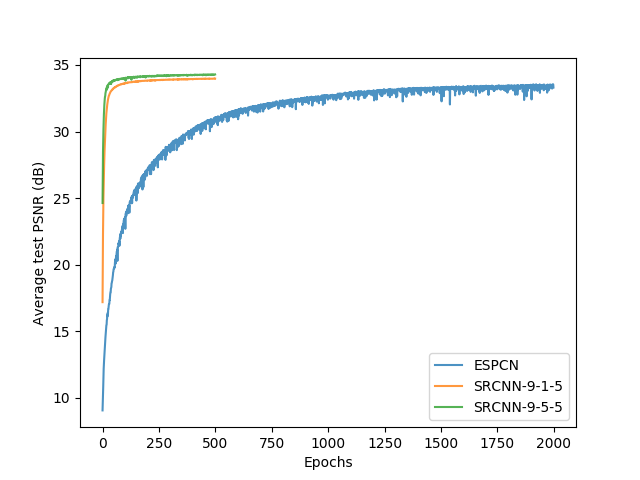
\includegraphics[width=2.5in]{history-sc3.png}
\caption{Scale 3 training history}
\label{fig_3}
\end{figure}

It's worth notice that in this plot the learning rate of ESPCN is $10^{-4}$ while SRCNN 's learning rate is $10^{-3}$, and it takes 2000 epochs for ESPCN to achieve the same PSNR as SRCNN indicating that ESPCN is much harder to learn than SRCNN. The same learning rate as SRCNN for ESPCN is too large as we can see in Fig. \ref{fig_4}. The PSNR is jumping around the minimum.

\begin{figure}[!t] 
\centering
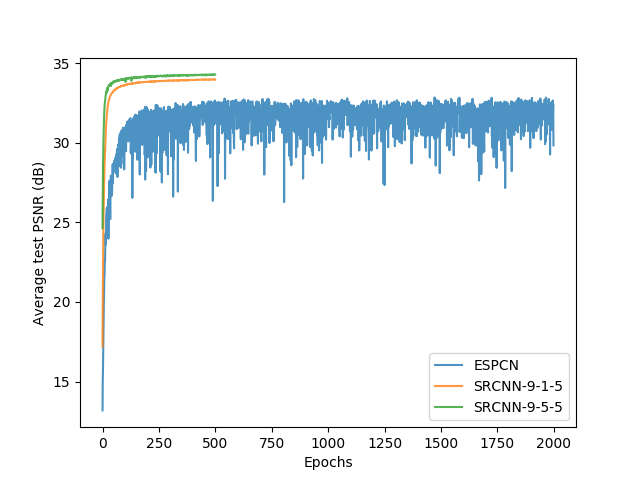
\includegraphics[width=2.5in]{history-sc3_largerrate.png}
\caption{ESPCN $10^{-3}$ learning rate}
\label{fig_4}
\end{figure}

\subsection{PSNR vs. Run Time}
The speed of predicting a HR image from a LR image determines whether it can be used in video and codec. The run time is the time it takes to make a HR prediction per LR image after the network has been trained. We test ESPCN, SRCNN 9-1-5, SRCNN 9-5-5, HEVC and Bicubic on two test set, one with 5 images, one with 14 images. The performance is shown in Fig. \ref{fig_5} and Fig. \ref{fig_6}.
As we can see in both results, SRCNN 9-5-5 have the highest PSNR while it's the slowest one except for HEVC. My implementation of HEVC interpolation use python and have no optimization while in the video coding standard they have specific hardware for this tasks. However, the performance of HEVC DCTIF is not as good as expected. The ESPCN is not only fast but also have great performance which is almost the same as SRCNN 9-5-5.
Apparently, there is a trade off between PSNR and Run Time. But ESPCN have the best overall performance although it's harder to train than SRCNN.


\begin{figure}[!t] 
\centering
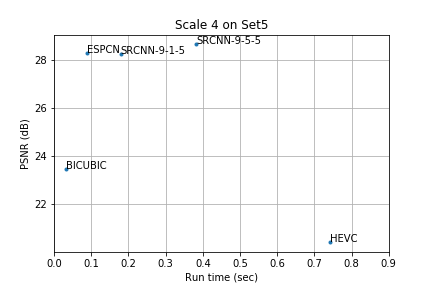
\includegraphics[width=2.5in]{performance-sc4-Set5.png}
\caption{Performance of scale 4 on Set5}
\label{fig_5}
\end{figure}

\begin{figure}[!t] 
\centering
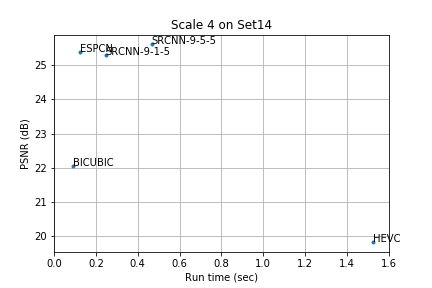
\includegraphics[width=2.5in]{performance-sc4-Set14.png}
\caption{Performance of scale 4 on Set14}
\label{fig_6}
\end{figure}


\subsection{Example}
In this section, Fig. \ref{fig_example} gives some example images used different method .
\begin{figure*}[!t]
\normalsize
\centering
\subfloat[original]{
	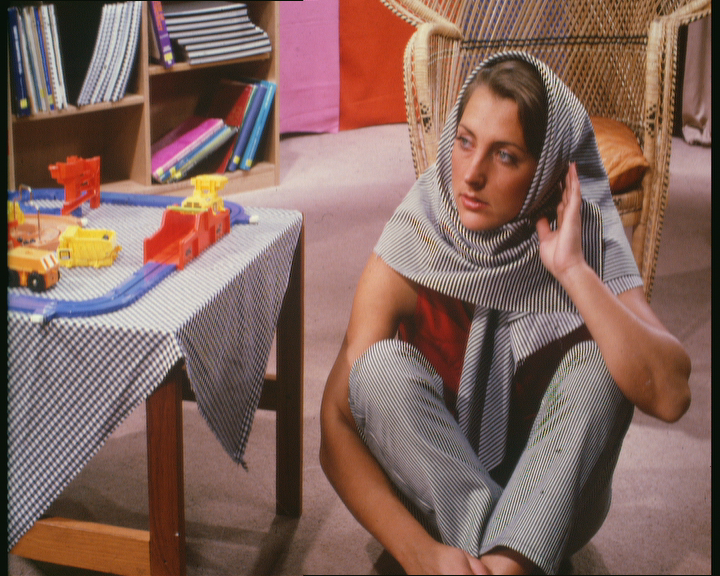
\includegraphics[width=2.5in]{barbara_original.png}
} 
\hfil 
\subfloat[down sampling input]{
	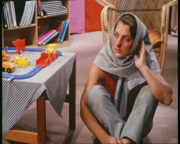
\includegraphics[width=2.5in]{barbara_input.png} 
	\label{fig_second_case}
}
\hfil 
\subfloat[SRCNN915]{
	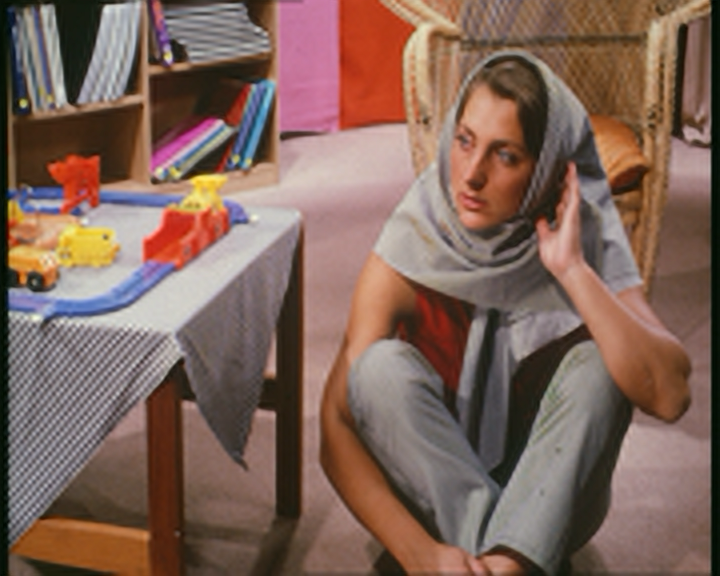
\includegraphics[width=2.5in]{barbara_SRCNN915.png} 
	\label{fig_second_case}
}
\hfil 
\subfloat[SRCNN955]{
	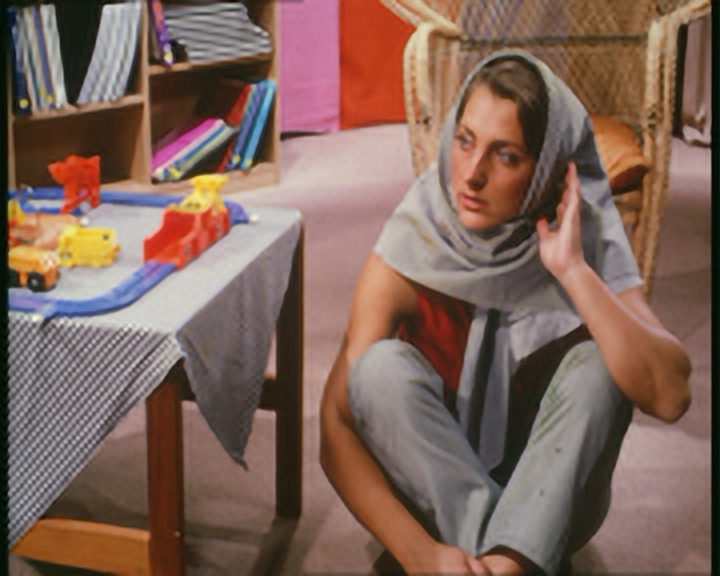
\includegraphics[width=2.5in]{barbara_SRCNN955.png} 
	\label{fig_second_case}
}
\hfil 
\subfloat[ESPCN]{
	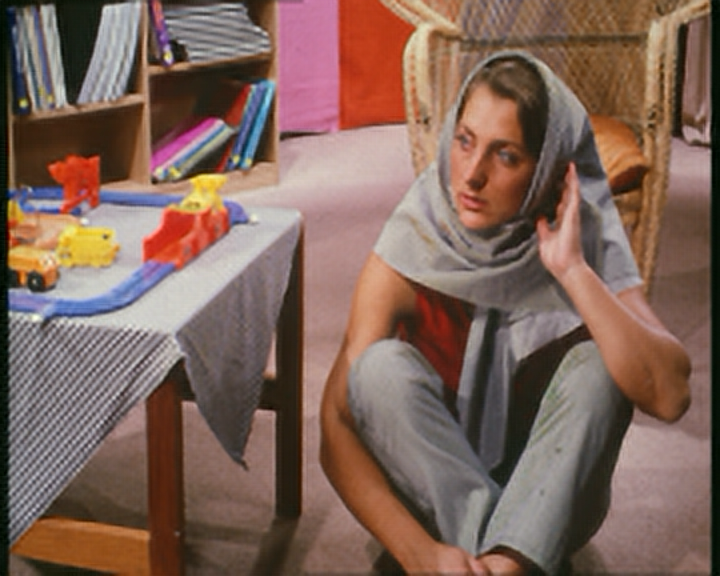
\includegraphics[width=2.5in]{barbara_espcn.png} 
	\label{fig_second_case}
}
\hfil 
\subfloat[Bicubic]{
	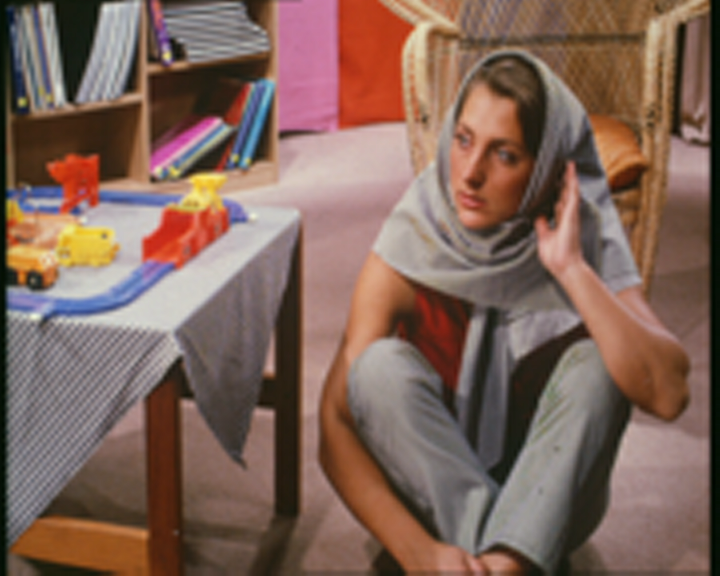
\includegraphics[width=2.5in]{barbara_bicubic.png} 
	\label{fig_second_case}
}
\hfil 
\subfloat[Bicubic]{
	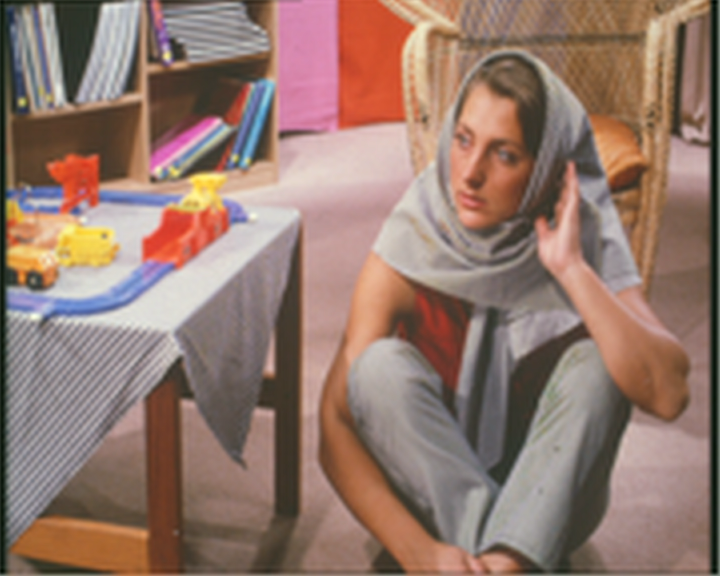
\includegraphics[width=2.5in]{barbara_hevc.png} 
	\label{fig_second_case}
}
\caption{Example images} 
\label{fig_example} 
\end{figure*}

\subsection{Discussion and Conclusions}
We have compared two different models of image super-resolution, SRCNN and ESPCN, with the traditional Bicubic and HEVC methods.

Both PSNR and run time of the SRCNN model scale with the number of parameters, as can be seen by comparing SRCNN 9-1-5 with SRCNN 9-5-5 where the latter has more parameters. SRCNN 9-5-5 is the best super-resolution among all the methods we tried. However, due to the upscaling (deconvolution) is at the front of the network. The speed is not fast enough to be useful for video super-resolution.

From ESPCN result, we know that there is a trade-off between quality (measured by PSNR) and run time. If the time cost is negligible, earlier deconvolution makes the HR image reconstruction better. 

All in all, ESPCN can achieved fast speed and relatively good performance. From the result we can see that HEVC interpolation isn't good enough. If we can use ESPCN in video codec for sub-pixel interpolation, the accuracy of motion estimation and motion compensation can be further improved.

\ifCLASSOPTIONcaptionsoff
  \newpage
\fi


\bibliography{refer.bib}
\bibliographystyle{ieeetr}





\end{document}


